\section{User Evaluation}
\label{sec:eval}
% We conducted a user evaluation to evaluate the effectiveness of our proposed pipeline and visual designs.
In this section, we introduce our evaluation methodology (\cref{sec:eval-method}), and report findings derived from the results (\cref{sec:eval-result}).


\subsection{Methodology}
\label{sec:eval-method}
To evaluate the effectiveness of our pipeline, we conducted a qualitative expert evaluation using {\tname} as a technology probe.
The evaluation had two goals:
firstly, to assess whether our approach is effective in assisting users in comprehending quantum circuits,
and secondly, to evaluate the usefulness of our visual designs in the analysis and optimization of large-scale quantum circuits.


\textbf{Participants.}
We recruited 10 quantum researchers (P1-P10; age: 22-30) from university quantum computing laboratories.
They included undergraduates, graduates, and professors from computer science and physics departments.
All participants majored in quantum computing with experience in developing quantum circuits (P1-P4: < 1 year, P5-P8: 1-4 years, P9-P10: > 8 years).
Their most frequently used visualization tool for quantum circuit is Qiskit.
Four of them (P3-4, P6-7) focused on small-scale circuits with up to 20 qubits, while the others had worked on larger circuits with more than 50 qubits.
We conducted online experiments that lasted 40 to 60 minutes. 
Each participant received approximately \$15 at the start of the session.

\textbf{Task.}
The participants were asked to complete three tasks using {\tname}: a training task (\textbf{T0}), a depiction task (\textbf{T1}), and an analysis task (\textbf{T2}).
For the depiction task, we prepared a quantum circuit with multi-level structure, and required participants to illustrate the backbone of the circuit using the resulting visualizations from the structure, component, and abstraction views.
The analysis task required participants to use context visualizations to analyze and find potential optimization in a quantum circuit.
The training task was prepared to cover all the features in \textbf{T1} and \textbf{T2}.
In total, we prepared six quantum circuits that represents different quantum algorithms, respectively.
Each circuit contains 30 to 99 qubits and over 10 hierarchical components.
We also provided the participants with a document that included the textual description and source code for the algorithms.

\textbf{Procedure.}
The study began with the introduction (10~min) of the study purpose, the motivation of improving quantum circuit representation, and the concepts in our proposed approach.
Next, we proceeded to the training task (\textbf{T0}, 15~min). 
We demonstrated the features of {\tname} with a quantum circuit and asked the experts to reproduce the process themselves.
After the training, we provided the experts with two quantum circuits for the two practical tasks (\textbf{T1} and \textbf{T2}, 10~min for each).
We ensured that the participants were not familiar with the circuit provided in \textbf{T1} and encouraged them to learn and ask questions about the quantum algorithms before starting the trial.
For each task, we asked the experts to depict at least two levels of structure and one visual abstraction.
Finally, the session ended with a semi-structured interview (15~min) and a post-study questionnaire (5-Point Likert Scale). 
% We collected their feedback on our system regarding to advantages, limitations, and potential improvements.
Each session was run in-lab following a think-aloud protocol.

\begin{figure}[tb]
    \centering
    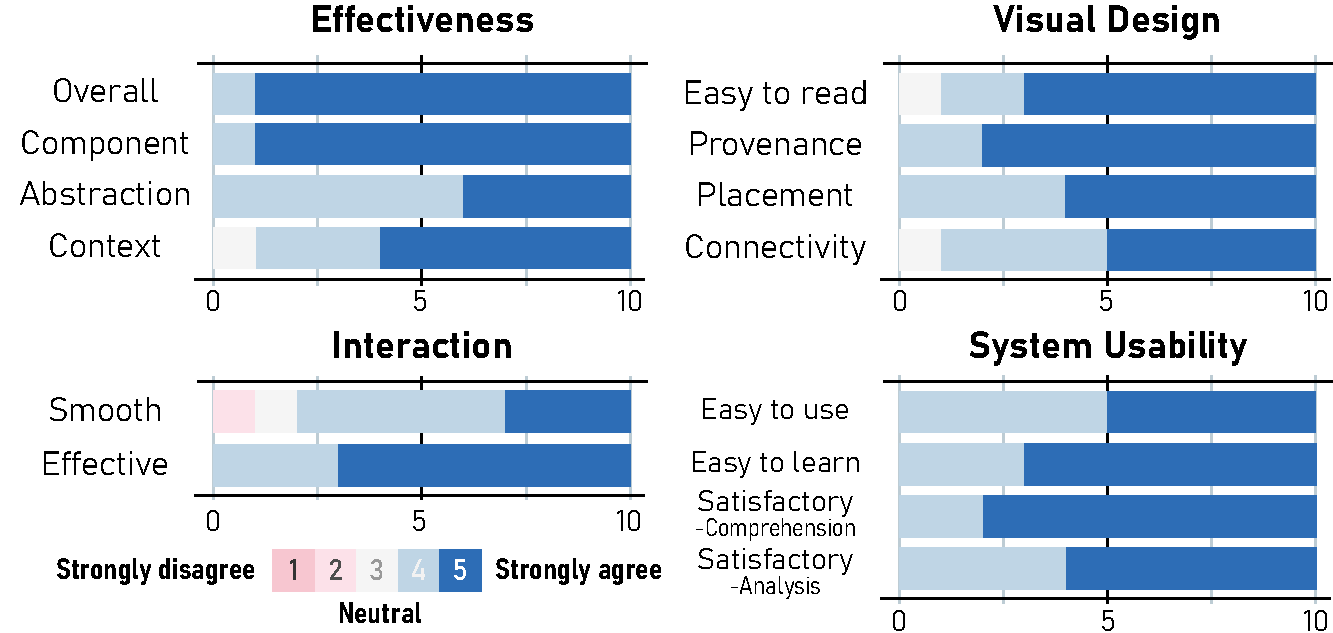
\includegraphics[width=\linewidth]{results}
    \caption{%
        User evaluation results.%
    }
    \label{fig:results}
\end{figure}


\subsection{Findings}
\label{sec:eval-result}
In summary, the evaluation results demonstrate a high level of user satisfaction and effectiveness of {\tname} in supporting quantum circuit exploration and analysis.
\Cref{fig:results} illustrates the results of our evaluation, and we provide a detailed analysis of the findings below. 

\textbf{Effectiveness.}
Participants appreciated the effectiveness of {\tname} in exploring and analyzing quantum circuits ($\mu$ = 4.7, $\sigma$ = 0.5). 
The \emph{Structure} and \emph{Component Views} were particularly praised for their ability to hierarchically outline the circuit, as well as the ability to customize the level of detail in the views.
Participants also noted the usefulness of \emph{Abstraction View} in identifying repetitive patterns, with P8 commenting that \emph{``it's easier to read a scalable circuit with abstractions''}.
Most participants believed the \emph{Context View} provided effective contextual information for circuit analysis, 
whilst some participants expressed the desire for more detailed indicators of the circuit, such as noises and parameters (P1,P3).
% \emph{``want to see more detailed indicators of the circuit, such as noises, parameters, and etc.''} 
Overall, \emph{Quantivine} was perceived as an effective tool for reducing the complexity of circuit representation, and was noted that \emph{``it eases the burden of interpreting circuits''} (P6).

\textbf{Visual Design.}
Participants rated {\tname} highly for its aesthetics, clarity, and usefulness of visual encoding ($\mu$ = 4.6, $\sigma$ = 0.6).
They responded that our design was visually appealing and easy to use.
Participants particularly appreciated the color-coding and highlighting of the placement view for its \emph{``clear and intuitive perception of global placement information''} (P3).
The \emph{Connectivity View} received mixed responses. 
While some participants were \emph{``not convinced''} (P2) due to their unfamiliarity with the matrix representation, other participants found \emph{``it's interesting to investigate the circuit using an adjacency matrix''} (P9) and obtained valuable insights from it.
One participant, P4, specifically noted the usefulness of the connectivity view in his current research about the entanglement analysis of quantum circuit.


\textbf{Interaction \& System Usability.}
Participants responded positively about the usability of {\tname} ($\mu$ = 4.7, $\sigma$ = 0.5), finding it easy to learn and use with fluent and efficient interactions ($\mu$ = 4.4, $\sigma$ = 0.8).
They expressed interest in using {\tname} to comprehend and explain other quantum algorithms in the future, as well as for circuit analysis and optimization.
Furthermore, two professors appreciated for the comprehensive views of quantum circuits provided by \emph{Quantivine}, and expressed interest in sharing the tool in their educational work, indicating its potential to contribute to the advancement of quantum computing education and research.


\textbf{Suggestions.}
Some participants suggested improvements to certain features, such as the ability to annotate and save their work within the tool.
P10 noted that the current system was targeted for the expert users, adding direct manipulation on the diagram, and synchronization with the source code may make it friendly to novice users.
P3 commented that he would be happy if {\tname} could additionally visualize the state of qubits in the intermediate or final stages of the execution.
